
In this appendix, we present in details our analytical study of {\sigmaFGM}. We assume that the reader is aware of the basic definitions and equations provided in the main manuscript.

%%%%%%%%%%%%%%%%%
%%%%%%%%%%%%%%%%%

\section*{Analytical study for a single phenotypic character}

In the single-character's version of {\sigmaFGM} ($n=1$), each organism owns two evolvable parameters $\mu \in \mathbb{R}$ and $\sigma \in \mathbb{R}_+$, encoding for the phenotypic distribution $z \sim \mathcal{N}(\mu,\sigma^2)$. The probability density to express the phenotype $z$ is:
\begin{equation}
p(z,\mu,\sigma) = \dfrac{1}{\sigma \sqrt{2\pi}} \exp \left[ \dfrac{-(z-\mu)^2}{2\sigma^2} \right].
\end{equation}
The fitness $W(z)$ of the expressed phenotype $z$ reads:
\begin{equation}
W(z) = \exp \left[ -z^2/2 \right].
\end{equation}
However, it is much more informative to look at the expected fitness $\overline{W}(\mu,\sigma)$ of an organism $(\mu,\sigma)$, that reads:
\begin{equation}
\begin{array}{rcl}
\overline{W}(\mu,\sigma) & = & \displaystyle\int_z p(z,\mu,\sigma)W(z)dz\\\\
& = & \displaystyle\int_z \dfrac{1}{\sigma \sqrt{2\pi}} \exp \left[ \dfrac{-(z-\mu)^2}{2\sigma^2} \right] \exp \left[ -\dfrac{z^2}{2} \right] dz.
\end{array}
\label{eq:part1:mean_fitness}
\end{equation}
We performed an analytical study of $\overline{W}(\mu,\sigma)$ in the space $(\mu,\sigma)$. We computed the partial derivatives $\partial \overline{W}(\mu,\sigma)/\partial \mu$ and $\partial \overline{W}(\mu,\sigma)/\partial \sigma$ in order to predict what would be the selective pressures on $\mu$ and $\sigma$, depending on the distance from the fitness optimum $z_{opt} = 0$. 

By way of introduction, we know that for $f$ continuously differentiable in $x$ and $t$, according to the Leibniz's rule:
\begin{equation}
\dfrac{d}{dt} \int_{\mathbb{R}} f(x,t)dx = \int_{\mathbb{R}} \dfrac{\partial}{\partial t} f(x,t) dx.
\label{eq:part1:leibniz_rule}
\end{equation}
Let us define the function $f(z,\mu,\sigma)$ such that:
\begin{equation}
f(z,\mu,\sigma) = p(z,\mu,\sigma)W(z)
\label{eq:part1:f_function}
\end{equation}

then:
\begin{equation}
\overline{W}(\mu,\sigma) = \displaystyle\int_{\mathbb{R}} f(z,\mu,\sigma)dz.
\label{eq:part1:int_f}
\end{equation}

%%%%%%%%%%%%%%%%%

\subsection*{Partial derivation on $\mu$}

According to Equations \ref{eq:part1:leibniz_rule} and \ref{eq:part1:int_f}, we know that:
\begin{equation}
\begin{array}{rcl}
\dfrac{\partial \overline{W}(\mu,\sigma)}{\partial \mu} & = & \displaystyle\int_z \dfrac{\partial}{\partial \mu} f(z,\mu,\sigma) dz.
\end{array}
\end{equation}

Let us compute $\partial f / \partial \mu$:

\begin{equation}
\begin{array}{rcl}
\dfrac{\partial f}{\partial \mu} & = & \dfrac{1}{\sigma \sqrt{2\pi}} \exp \left[ -\dfrac{z^2}{2} \right] \left(\exp \left[ \dfrac{-(z-\mu)^2}{2\sigma^2} \right] \right)'\\\\
& = & \dfrac{1}{\sigma \sqrt{2\pi}} \exp \left[ -\dfrac{z^2}{2} \right] \dfrac{(z-\mu)}{\sigma^2} \exp \left[ \dfrac{-(z-\mu)^2}{2\sigma^2} \right]\\\\
& = & \dfrac{(z-\mu)}{\sigma^2} f(z,\mu,\sigma)\\\\
& = & \dfrac{(z-\mu)}{\sigma^2} p(z,\mu,\sigma)W(z)
\end{array}
\label{eq:part1:mu_derivation}
\end{equation}

$p(z,\mu,\sigma)$ being a Gaussian density, we know that:
\begin{equation}
\dfrac{\partial p(z,\mu,\sigma)}{\partial z} = -\dfrac{(z-\mu)}{\sigma^2}\ p(z,\mu,\sigma).
\end{equation}

Then, Equation \ref{eq:part1:mu_derivation} can be rewritten as following:
\begin{equation}
\dfrac{\partial f(z,\mu,\sigma)}{\partial \mu} = -\dfrac{\partial p(z,\mu,\sigma)}{\partial z}W(z).
\end{equation}

Here, the goal here is to determine the sign of $\partial \overline{W}(\mu,\sigma)/\partial \mu$, that reads:
\begin{equation}
\begin{array}{rcl}
\dfrac{\partial \overline{W}(\mu,\sigma)}{\partial \mu} & = & \displaystyle\int_z \dfrac{\partial f(z,\mu,\sigma)}{\partial \mu} dz\\\\
& = & \displaystyle\int_z \underbrace{-\dfrac{\partial p(z,\mu,\sigma)}{\partial z}}_{\text{Anti-symmetric function}} \times \underbrace{W(z)}_{\text{Symmetric function}} dz.
\end{array}
\label{eq:part1:mu_full_equation}
\end{equation}

To determine the sign of $\partial \overline{W}(\mu,\sigma)/\partial \mu$, we must consider the shape of the integrated function, being the product of:
\begin{enumerate}
\item[\textbf{(1)}] $-\partial p(z,\mu,\sigma)/\partial z$, an anti-symmetric function centered on $\mu$, negative if $z < \mu$, and positive if $z > \mu$ (Fig. \ref{part1:appendixS3:fig1}a);
\item[\textbf{(2)}] $W(z)$, a strictly positive and symmetric function, centered on 0  (Fig. \ref{part1:appendixS3:fig1}b).
\end{enumerate}

When $\mu=0$, the product of the anti-symmetric and symmetric functions $\partial p(z,\mu,\sigma)/\partial z \times W(z)$ is an anti-symmetric function, its integral thus being equal to zero (Figs. \ref{part1:appendixS3:fig1}c and \ref{part1:appendixS3:fig1}d). Then, the sign of $\partial \overline{W}(\mu,\sigma)/\partial \mu$ depends on $\mu$ as following:
\begin{equation}
\left\{
\begin{array}{rcl}
\text{If } \mu < 0 &,& \partial f(z,\mu,\sigma)/\partial \mu > 0\\\\
\text{If } \mu = 0 &,& \partial f(z,\mu,\sigma)/\partial \mu = 0\\\\
\text{If } \mu > 0 &,& \partial f(z,\mu,\sigma)/\partial \mu < 0
\end{array}
\right.
\end{equation}

Hence, for any value of $\sigma > 0$, the selective pressures act to reduce $\mu$ towards $\mu=0$, defining a ridge $\partial \overline{W}(\mu,\sigma)/\partial \mu = 0$ when $\mu = 0$. Any organism owning a value of $\mu \neq 0$ has a lower fitness than an organism with $\mu = 0$, for any given value of $\sigma$. This ridge is plotted in purple on Figure \ref{part1:appendixS3:fig3}.

As revealed in Equation \ref{eq:part1:mu_derivation}, two other conditions exist for $\partial W(\mu,\sigma)/\partial \mu = 0$:
\begin{equation}
\left\{
\begin{array}{rcl}
\text{If } \mu \rightarrow \pm \infty &,& \partial f(z,\mu,\sigma)/\partial \mu = 0\\\\
\text{If } \sigma \rightarrow +\infty &,& \partial f(z,\mu,\sigma)/\partial \mu = 0\\\\
\end{array}
\right.
\end{equation}

Thus, organisms located very far from the fitness optimum (\textit{i.e.}, $|\mu| \gg 0$), or organisms with a very dispersed phenotypic distribution (\textit{i.e.}, $\sigma \gg 0$), do not experience selective pressures. However, according to Equation \ref{eq:part1:mean_fitness}, their mean fitness $\overline{W}(\mu, \sigma)$ is almost equal to zero in these conditions.

Another critical condition to clarify for the partial derivative $\partial \overline{W}(\mu,\sigma)/\partial \mu$ is when $\sigma \rightarrow 0$. Equation \ref{eq:part1:mu_full_equation} can help us to solve this special case. Indeed, normal distributions with parameters $\mu$ and $\sigma$ converge towards a Dirac distribution $\delta(z-\mu)$ when $\sigma \rightarrow 0$. The Dirac distribution satisfies, for all continuous function $\varphi(z)$,
\begin{equation}
\int_z \delta(z-\mu)\varphi(z)dz = \varphi(\mu).
\end{equation}

The first derivative of the Dirac distribution (in the sense of distributions) satisfies:
\begin{equation}
\displaystyle\int_{\mathbb{R}} \delta'(z-\mu)\varphi(z)dz = -\varphi'(\mu)
\end{equation}
and the $n$-th derivative, denoted $\delta^{(n)}$, satisfies:
\begin{equation}
\displaystyle\int_z \delta^{(n)}(z-\mu) \varphi(z) dz = (-1)^n \varphi^{(n)}(\mu).
\end{equation}
 
Thus, starting from Equation \ref{eq:part1:mu_full_equation}, we can derive the following limiting equation when $\sigma \rightarrow 0$:
\begin{equation}
\begin{array}{rcl}
\lim\limits_{\sigma \to 0}\ \dfrac{\partial \overline{W}}{\partial \mu} & = & \lim\limits_{\sigma \to 0}\ \dfrac{\partial}{\partial \mu} \displaystyle\int_{\mathbb{R}} p(z,\mu,\sigma)W(z)dz\\\\
& = & \dfrac{\partial}{\partial \mu} \lim\limits_{\sigma \to 0}\ \displaystyle\int_{\mathbb{R}} p(z,\mu,\sigma)W(z)dz\\\\
& = & \dfrac{\partial}{\partial \mu} \displaystyle\int_{\mathbb{R}} \delta(z-\mu)W(z)dz\\\\
& = & \dfrac{\partial W(\mu)}{\partial \mu}\\\\
& = & W'(\mu).
\end{array}
\label{eq:part1:sigma_zero_limit}
\end{equation}

Thus, when $\sigma \rightarrow 0$, the system converges towards canonical FGM scenario, according that $\mu \equiv z$ in this case.

%%%%%%%%%%%%%%%%%

\subsection*{Partial derivation on $\sigma$}

We first rewrite the equation $f(z,\mu,\sigma)$ to separate $\sigma$ from other terms:
\begin{equation}
f(z,\mu,\sigma) = \dfrac{W(z)}{\sqrt{2\pi}} \times \dfrac{1}{\sigma} \exp \left[\dfrac{-(z-\mu)^2}{2\sigma^2}\right].
\end{equation}
Let us define the term $a = W(z)/\sqrt{2\pi}$ that does not depend on $\sigma$, such that:
\begin{equation}
f(z,\mu,\sigma) = a \times \dfrac{1}{\sigma} \exp \left[\dfrac{-(z-\mu)^2}{2\sigma^2}\right].
\end{equation}

The partial derivation of $f$ with respect to $\sigma$ is more technical than for $\mu$. We describe it step by step below.
Let us define the terms $u$ and $v$ such that:
\begin{equation}
\left\{
\begin{array}{rcl}
u & = & \exp \left[\dfrac{-(z-\mu)^2}{2\sigma^2} \right]\\\\
v & = & \sigma
\end{array}
\right.
\end{equation}
Then:
\begin{equation}
\dfrac{\partial f(z,\mu,\sigma)}{\partial \sigma} = a \times \dfrac{(u'v-uv')}{v^2}
\end{equation}
with:
\begin{equation}
\left\{
\begin{array}{rcl}
u' & = & \dfrac{(z-\mu)^2}{\sigma^3} \exp \left[\dfrac{-(z-\mu)^2}{2\sigma^2} \right]\\\\
v' & = & 1
\end{array}
\right.
\end{equation}

Thus, the derivative $\partial f/\partial \sigma$ reads:
\begin{equation}
\begin{array}{rcl}
\dfrac{\partial f(z,\mu,\sigma)}{\partial \sigma} & = & a \times \left( \dfrac{\dfrac{\sigma(z-\mu)^2}{\sigma^3} \exp \left[\dfrac{-(z-\mu)^2}{2\sigma^2}\right] - \exp \left[\dfrac{-(z-\mu)^2}{2\sigma^2}\right]}{\sigma^2}\right)\\\\
& = & a \times \exp \left[\dfrac{-(z-\mu)^2}{2\sigma^2}\right] \times \left( \dfrac{\dfrac{(z-\mu)^2}{\sigma^2} - 1}{\sigma^2}\right)\\\\
& = & a \times \exp \left[\dfrac{-(z-\mu)^2}{2\sigma^2}\right] \times \dfrac{(z-\mu)^2-\sigma^2}{\sigma^4}\\\\
& = & \dfrac{(z-\mu)^2-\sigma^2}{\sigma^3}\ f(z,\mu,\sigma)\\\\
& = & \dfrac{(z-\mu)^2-\sigma^2}{\sigma^3}\ p(z,\mu,\sigma)W(z)\\\\
\end{array}
\label{eq:part1:sigma_derivative}
\end{equation}

$p(z)$ being the density of a normal law, we know that:
\begin{equation}
\dfrac{\partial^2 p(z,\mu,\sigma)}{\partial z^2} = \dfrac{(z-\mu)^2-\sigma^2}{\sigma^4}\ p(z,\mu,\sigma).
\end{equation}

From Equation \ref{eq:part1:sigma_derivative}, we thus find:
\begin{equation}
\dfrac{\partial f(z,\mu,\sigma)}{\partial \sigma} = \underbrace{\dfrac{\partial^2 p(z,\mu,\sigma)}{\partial z^2}}_{\text{Symmetric function}} \times \underbrace{\sigma\ W(z)}_{\text{Symmetric function}}.
\end{equation}

We were not able to compute the ridge $\partial \overline{W}(\mu,\sigma)/\partial \sigma=0$. We used a numerical scheme to compute $\partial \overline{W}(\mu,\sigma)/\partial \sigma$ depending on $\mu$ and $\sigma$ (see Appendix \ref{part1:AppendixS2}).

However, it is possible to determine analytically some essential characteristics of the ridge $\partial \overline{W}(\mu,\sigma)/\partial \sigma=0$ (Fig. \ref{part1:appendixS3:fig3} orange curve):
\begin{enumerate}
\item[\textbf{(1)}] The sign of $\partial \overline{W}(\mu,\sigma)/\partial \sigma$ when $\sigma \rightarrow 0$;
\item[\textbf{(2)}] The position of the inflection point $\mu=d_{th}$, below which the phenotypic noise is always deleterious (Fig. \ref{part1:appendixS3:fig3} orange circle).
\end{enumerate}

\paragraph{(1)}
As previously (Eq. \ref{eq:part1:sigma_zero_limit}), when $\sigma \rightarrow 0$, $\partial \overline{W}(\mu,\sigma)/\partial \sigma$ reads:
\begin{equation}
\begin{array}{rcl}
\lim\limits_{x \to 0}\ \dfrac{\partial \overline{W}(\mu,\sigma)}{\partial \sigma} & = & \displaystyle\int_z \delta^{''}(z-\mu) \times \sigma\ W(z) dz\\\\
& = & (-1)^2 \sigma\ W^{''}(\mu)\\\\
& = & \sigma (\mu^2-1) \ W(\mu)\\\\
& = & 0.
\end{array}
\end{equation}

Thus, when $\sigma \rightarrow 0$, the first order selective pressure on $\sigma$ vanishes, for any values of $\mu$. This means that to determine whether low noise levels are beneficial, one must look at the second derivative of $\overline{W}$ with respect to $\sigma$, and identify the inflection points that separate the regions where noise is beneficial or deleterious.

\paragraph{(2)}

We first compute $\partial^2 f/\partial \sigma^2$. From Equation \ref{eq:part1:sigma_derivative}, we define the terms $u$ and $v$ such that:
\begin{equation}
\left\{
\begin{array}{rcl}
u & = & \dfrac{(z-\mu)^2-\sigma^2}{\sigma^3}\\\\
v & = & f(z,\mu,\sigma)
\end{array}
\right.
\end{equation}

Thus, $\partial^2 f/\partial \sigma^2 = u'v+uv'$, with:
\begin{equation}
\begin{array}{rcl}
u' & = & \dfrac{\sigma^2-3(z-\mu)^2}{\sigma^4}\\\\
v' & = & \dfrac{(z-\mu)^2-\sigma^2}{\sigma^3} f(z,\mu,\sigma)
\end{array}
\end{equation}

%%%%%%%%%%%%%%%%%%%%%%%%%%%%%%%%%%%%%%%%%%%%
% FIGURES
%%%%%%%%%%%%%%%%%%%%%%%%%%%%%%%%%%%%%%%%%%%%

\begin{figure}[!h]
\begin{adjustwidth}{-0in}{0in}
\centering
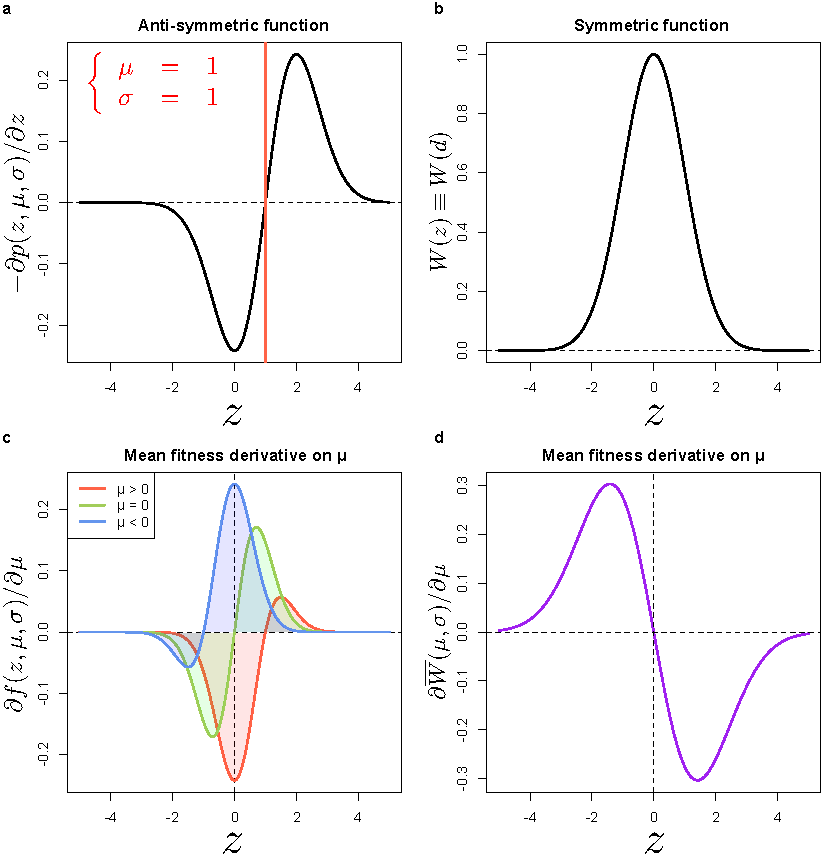
\includegraphics[scale=1]{part1_appendixS3_fig1.pdf}
\end{adjustwidth}
\caption[Behavior of $\partial \overline{W}(\mu,\sigma)/\partial \mu$.]{
\textbf{Behavior of $\partial \overline{W}(\mu,\sigma)/\partial \mu$.}
\textbf{a,} The normal distribution derivative $-\partial p(z,\mu,\sigma)/\partial z$ is an anti-symmetric function centered on $z=\mu$, such that the function is negative when $z < \mu$ and positive when $z > \mu$. Here, an example is given for $\mu=1$ and $\sigma=1$. The red vertical line represents the value of $\mu$, which is an axis of symmetry of the function.
\textbf{b,} The Gaussian-shaped fitness function $W(z)$ is a strictly positive, symmetric function centered on $z=0$.
\textbf{c,d,} The product of both functions, equal to $\partial f(z,\mu,\sigma)/\partial \mu$ is biased towards positive values if $\mu < 0$ (blue curve), towards negative values if $\mu > 0$ (red curve), or anti-symmetric if $\mu=0$ (green curve). Thus the integral $\int_z \partial f(z,\mu,\sigma)/\partial \mu\ dz$ is respectively positive, negative, or zero, if $\mu$ is negative, positive or zero (as shown in panel \textbf{d}, purple curve).
}
\label{part1:appendixS3:fig1}
\end{figure}

\begin{figure}[!h]
\begin{adjustwidth}{-0in}{0in}
\centering
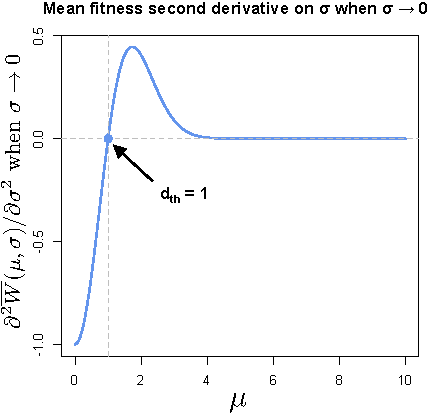
\includegraphics[scale=1]{part1_appendixS3_fig2.pdf}
\end{adjustwidth}
\caption[Variation of $\partial^2 W(\mu,\sigma)/\partial \sigma^2$ when $\sigma \rightarrow 0$.]{
\textbf{Variation of $\partial^2 \overline{W}(\mu,\sigma)/\partial \sigma^2$ when $\sigma \rightarrow 0$.}
The variation of $\partial^2 \overline{W}(\mu,\sigma)/\partial \sigma^2$ when $\sigma \rightarrow 0$ is represented here depending on $\mu$. It is described by Equation \ref{eq:part1:d2wdsigma}. Blue dot: inflection point of the ridge $\partial \overline{W}(\mu,\sigma)/\partial \sigma = 0$ (Fig. \ref{part1:appendixS3:fig3} orange circle), for $\mu = d_{th} = 1$.
}
\label{part1:appendixS3:fig2}
\end{figure}

\begin{figure}[!h]
\begin{adjustwidth}{-0in}{0in}
\centering
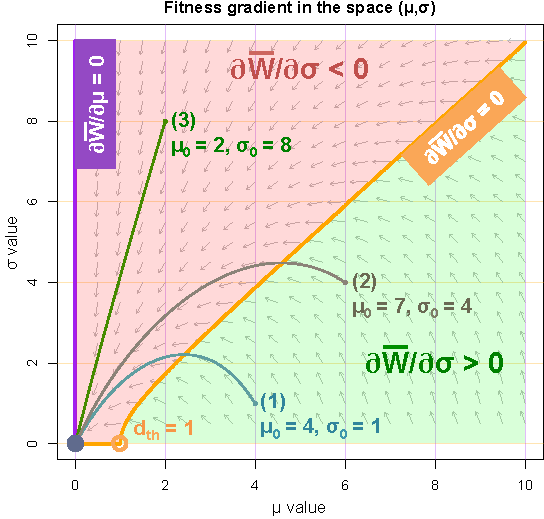
\includegraphics[scale=1]{part1_appendixS3_fig3.pdf}
\end{adjustwidth}
\caption[Variations of the mean fitness $\overline{W}(\mu,\sigma)$ in the space $(\mu,\sigma)$.]{\textbf{Variations of the mean fitness $\overline{W}(\mu,\sigma)$ in the space $(\mu,\sigma)$.}
In purple, the ridge $\partial \overline{W}/\partial \mu=0$. In orange, the ridge $\partial \overline{W}/\partial \sigma=0$. Green area: $\partial \overline{W}/\partial \sigma > 0$ (\textit{i.e.}, it is beneficial to increase the phenotypic noise). Red area: $\partial \overline{W}/\partial \sigma < 0$ (\textit{i.e.}, it is beneficial to reduce the phenotypic noise). Three trajectories following the fitness gradient are represented \textbf{(1)} in blue (initial values: $\mu_0=4, \sigma_0=1$), \textbf{(2)} in brown (initial values: $\mu_0=6, \sigma_0=4$) and \textbf{(3)} in green (initial values: $\mu_0=2, \sigma_0=8$). Black dot: fitness optimum $z_{opt}$. Orange circle: inflection point $d_{th}=1$ of the fitness landscape $W(z)$. Grey arrows indicate the direction of the fitness gradient, but not its amplitude.
}
\label{part1:appendixS3:fig3}
\end{figure}

%%%%%%%%%%%%%%%%%%%%%%%%%%%%%%%%%%%%%%%%%%%%
%%%%%%%%%%%%%%%%%%%%%%%%%%%%%%%%%%%%%%%%%%%%

The second derivative of $f$ then reads:
\begin{equation}
\begin{array}{rcl}
\dfrac{\partial^2 f(z,\mu,\sigma)}{\partial \sigma^2} & = & \dfrac{(z-\mu)^2-\sigma^2}{\sigma^3} f(z,\mu,\sigma) + \left( \dfrac{\sigma^2-3(z-\mu)^2}{\sigma^4}\right)^2 f(z,\mu,\sigma)\\\\
& = & f(z,\mu,\sigma) \left( \dfrac{\sigma^4-3\sigma^2(z-\mu)^2+(z-\mu)^4-2(z-\mu)^2\sigma^2+\sigma^4}{\sigma^6} \right)\\\\
& = & f(z,\mu,\sigma) \left( \dfrac{2\sigma^4-5(z-\mu)^2\sigma^2+(z-\mu)^4}{\sigma^6} \right).
\end{array}
\end{equation}
As demonstrated previously, it is possible to rewrite this equation to extract derivatives of normal law densities:
\begin{equation}
\begin{array}{rcl}
\dfrac{\partial^2 f(z,\mu,\sigma)}{\partial \sigma^2} & = & f(z,\mu,\sigma) \left( \dfrac{(z-\mu)^4-6(z-\mu)^2\sigma^2+3\sigma^4}{\sigma^6}+\dfrac{(z-\mu)^2\sigma^2-\sigma^4}{\sigma^6} \right)\\\\
& = & \sigma^2\ f(z,\mu,\sigma) \left( \dfrac{(z-\mu)^4-6(z-\mu)^2\sigma^2+3\sigma^4}{\sigma^8} + \dfrac{1}{\sigma^2}\dfrac{(z-\mu)^2-\sigma^2}{\sigma^4} \right)\\\\
& = & \sigma^2\ f(z,\mu,\sigma) \left( \dfrac{(z-\mu)^4-6(z-\mu)^2\sigma^2+3\sigma^4}{\sigma^8} + \dfrac{(z-\mu)^2-\sigma^2}{\sigma^6} \right)\\\\
& = & \sigma^2\ W(z) \left( \dfrac{\partial^4 p(z,\mu,\sigma)}{\partial z^4} + \dfrac{1}{\sigma^2} \times \dfrac{\partial^2 p(z,\mu,\sigma)}{\partial z^2} \right)\\\\
& = & \underbrace{\left( \sigma^2\ W(z) \dfrac{\partial^4 p(z,\mu,\sigma)}{\partial z^4} \right)}_{\rightarrow 0 \text{ when } \sigma \rightarrow 0} + \left(W(z) \dfrac{\partial^2 p(z,\mu,\sigma)}{\partial z^2} \right).
\end{array}
\label{eq:part1:second_derivative}
\end{equation}

Consequently, when $\sigma \rightarrow 0$, the partial derivative $\partial^2 \overline{W}(\mu,\sigma)/\partial \sigma^2$ reads:
\begin{equation}
\lim\limits_{x \to 0}\ \dfrac{\partial^2 \overline{W}(\mu,\sigma)}{\partial \sigma^2} = (\mu^2-1)\ W(\mu).
\label{eq:part1:d2wdsigma}
\end{equation}

The only value of $\mu$ for which $\partial^2 \overline{W}(\mu,\sigma)/\partial \sigma^2 = 0$ is $|\mu| = 1$. When $|\mu| < 1$, $\partial^2 \overline{W}(\mu,\sigma)/\partial \sigma^2 < 0$, meaning that the selective pressure is towards a reduction of the phenotypic noise $\sigma$. When $|\mu| > 1$, $\partial^2 \overline{W}(\mu,\sigma)/\partial \sigma^2 > 0$, meaning that the selective pressure is towards an increase of the phenotypic noise $\sigma$ (Fig. \ref{part1:appendixS3:fig2} blue curve, and Fig. \ref{part1:appendixS3:fig3} orange curve and circle). Thus, $d_{th}=1$.

%%%%%%%%%%%%%%%%%
%%%%%%%%%%%%%%%%%

\section*{Analytical and numerical studies of an isotropic noise on $n$ phenotypic characters}

As described in Results, an isotropic noise is applied to the mean phenotype $\boldsymbol{\mu}$, by independently varying each trait value $\mu_i$ with the same noise amplitude $\sigma$. The probability $p(\boldsymbol{z},\boldsymbol{\mu},\sigma)$ for an organism $(\boldsymbol{\mu}, \sigma)$ to express the phenotype $\boldsymbol{z}$ is then:
\begin{equation}
p(\boldsymbol{z},\boldsymbol{\mu},\sigma) = \prod_{i \in n} \dfrac{1}{\sigma \sqrt{2\pi}} \exp \left[ \dfrac{-(z_i-\mu_i)^2}{2\sigma^2} \right].
\end{equation}

As in the previous section, the goal is to compute the second derivative of $\overline{W}(\boldsymbol{\mu}, \sigma)$ on $\sigma$, and find its inflection point to detect the critical euclidean distance $d_{th}$ below which phenotypic noise must be minimized. However, we now must compute it in $n$ dimensions. Hopefully, two conditions allow us to strongly simplify the equations:
\begin{enumerate}
\item[\textbf{(1)}] Noise is isotropic, such that $\overline{W}(\boldsymbol{\mu}, \sigma)$ can be decomposed in a product of one-dimensional integrals;
\item[\textbf{(2)}] The mean phenotype of an organism $\boldsymbol{\mu}$ is taken away from the fitness optimum on a single axis, all other axes remaining at a distance zero of the fitness optimum. By rotational symmetry, we can generalize to any position $\boldsymbol{\mu}$ away from the fitness optimum.
\end{enumerate}

$\overline{W}(\boldsymbol{\mu}, \sigma)$ reads:
\begin{equation}
\begin{array}{rcl}
\overline{W}(\boldsymbol{\mu}, \sigma) & = & \displaystyle\int_{\mathbb{R}^n} p(\boldsymbol{z},\boldsymbol{\mu},\sigma)W(\boldsymbol{z})d\boldsymbol{z}\\\\
& = & \displaystyle\int_{\mathbb{R}} p(z_1,\mu_1,\sigma)W(z_1)dz_1 \times ... \times \displaystyle\int_{\mathbb{R}} p(z_n,\mu_n,\sigma)W(z_n)dz_n.
\end{array}
\end{equation}

If we only move the mean phenotypic trait value $\mu_1$ away from the fitness optimum, all other mean trait values being equal to zero, $\overline{W}(\boldsymbol{\mu}, \sigma)$ then reads:
\begin{equation}
\begin{array}{rcl}
\overline{W}(\boldsymbol{\mu}, \sigma) & = & \displaystyle\int_{\mathbb{R}} p(z_1,\mu_1,\sigma)W(z_1)dz_1 \times \left( \displaystyle\int_{\mathbb{R}} p(z,0,\sigma)W(z)dz \right)^{n-1}.
\end{array}
\end{equation}

As demonstrated above, we know that for a single character and when $\sigma \rightarrow 0$, the successive derivatives of $\overline{W}(\mu, \sigma)$ read:
\begin{equation}
\left\{
\begin{array}{ccl}
\overline{W} & = & W(\mu)\\\\
\overline{W}' & = & 0\\\\
\overline{W}'' & = & (\mu^2-1)W(\mu)
\end{array}
\right.
\label{eq:part1:derivative1}
\end{equation}

Moreover, when $\mu = 0$, we find that:
\begin{equation}
\left\{
\begin{array}{ccl}
\overline{W}_0 & = & 1\\\\
\overline{W}_0' & = & 0\\\\
\overline{W}_0'' & = & -1
\end{array}
\right.
\label{eq:part1:derivative2}
\end{equation}

We then define the terms $a$, $b$ and $c$ such that:
\begin{equation}
\left\{
\begin{array}{ccl}
a & = & \displaystyle\int_{\mathbb{R}} p(z_1,\mu_1,\sigma)W(z_1)dz_1\\\\
b & = & \displaystyle\int_{\mathbb{R}} p(z,0,\sigma)W(z)dz\\\\
c & = & b^{\ n-1}
\end{array}
\right.
\end{equation}

We now compute the second derivative of $\overline{W}(\boldsymbol{\mu}, \sigma)$ on $\sigma$, according to $a$, $b$ and $c$, this equation reads:
\begin{equation}
\dfrac{\partial^2 \overline{W}(\boldsymbol{\mu}, \sigma)}{\partial \sigma^2} = ac'' + 2a'c' + a''c
\end{equation}
With:
\begin{equation}
\left\{
\begin{array}{ccl}
c' & = & (n-1)b'b^{\ n-2}\\\\
c'' & = & (n-1)(n-2)b'b^{\ n-3} + (n-1)b''b^{\ n-2}
\end{array}
\right.
\end{equation}

Then, the complete equation of $\partial \overline{W}(\boldsymbol{\mu}, \sigma) / \partial \sigma$ reads:
\begin{equation}
\begin{array}{rcl}
\dfrac{\partial^2 \overline{W}(\boldsymbol{\mu}, \sigma)}{\partial \sigma^2} & = & a \left( (n-1)(n-2)b'b^{\ n-3} + (n-1)b''b^{\ n-2} \right)\\\\
& + & 2a'(n-1)b'b^{\ n-2}\\\\
& + & a''b^{\ n-1}.
\end{array}
\end{equation}

We now replace the terms $a$ and $b$ by the corresponding terms in Equations \ref{eq:part1:derivative1} and \ref{eq:part1:derivative2}:

\begin{equation}
\begin{array}{rcl}
\dfrac{\partial^2 \overline{W}(\boldsymbol{\mu}, \sigma)}{\partial \sigma^2} & = & \overline{W} \left( (n-1)(n-2)\overline{W}_0'\overline{W}_0^{\ n-3} + (n-1)\overline{W}_0''\overline{W}_0^{\ n-2} \right)\\\\
& + & 2\overline{W}'(n-1)\overline{W}_0'\overline{W}_0^{\ n-2}\\\\
& + & \overline{W}''\overline{W}_0^{\ n-1}.
\end{array}
\end{equation}

Finally, the second derivative of $\overline{W}(\boldsymbol{\mu}, \sigma)$ on $\sigma$ reads:
\begin{equation}
\dfrac{\partial^2 \overline{W}(\boldsymbol{\mu}, \sigma)}{\partial \sigma^2} = (\mu_1^2-n)W(\mu_1).
\label{eq:part1:super_equation}
\end{equation}

The only value of $\mu_1$ for which Equation \ref{eq:part1:super_equation} is equal to zero is $\mu_1 = \pm \sqrt{n}$. Since this result is valid when the euclidean distance $d = \lVert \boldsymbol{\mu} \rVert$ is equal to $\sqrt{n}$, we can conclude that the critical distance below which isotropic phenotypic noise must be minimized is $d_{th} = \sqrt{n}$.

%%%%%%%%%%%%%%%%%
%%%%%%%%%%%%%%%%%

\section*{Anisotropic and correlated phenotypic noise is beneficial when aligned with the fitness optimum}

Let us consider the organism $(\boldsymbol{\mu}, \boldsymbol{\sigma}, \boldsymbol{\theta})$ in a $n$-dimensional phenotypic space, sitting at a certain distance of the fitness optimum $\boldsymbol{z_{opt}}$ (beyond $d_{th}=\sqrt{n}$) and evolving towards it. We describe the phenotypic noise of this organism by a multivariate normal distribution $\mathcal{N}_n(\boldsymbol{\mu},\boldsymbol{\Sigma})$. This multivariate normal distribution can be represented by an hyper-ellipse in $\mathbb{R}^n$, as shown in Figure \ref{part1:appendixS3:fig4} for two dimensions.

We now define the axes $\boldsymbol{v_1}, ..., \boldsymbol{v_n}$ (the origin of the new basis also being $\boldsymbol{\mu}$), with $\boldsymbol{v_1}$ aligned towards the fitness optimum $\boldsymbol{z_{opt}}$, all other axes $\boldsymbol{v_i}$ being orthogonal to $\boldsymbol{v_1}$ (Fig. \ref{part1:appendixS3:fig4}a).
Along axis $\boldsymbol{v_1}$, the organism $(\boldsymbol{\mu}, \boldsymbol{\sigma}, \boldsymbol{\theta})$ experiences a convex fitness if $\lVert \boldsymbol{\mu} \rVert > 1$. Along all other axes $\boldsymbol{v_i}$, the organism experiences a concave fitness, sitting at a local optimum in all cases (Fig. \ref{part1:appendixS3:fig4}b).
The basis associated to axes $\boldsymbol{v_1}, ..., \boldsymbol{v_n}$ is the orthonormal matrix $\boldsymbol{V}$ of size $n \times n$, where $\boldsymbol{v_1}$ is defined by the vector $\boldsymbol{\mu}$. By defining $\overline{\boldsymbol{\mu}} = \boldsymbol{\mu}/\lVert \boldsymbol{\mu} \rVert$, the matrix $\boldsymbol{V}$ reads:
\begin{equation}
\boldsymbol{V} = 
\begin{pmatrix}
\left. \overline{\boldsymbol{\mu}} \right| ... 
\end{pmatrix}
\end{equation}

The goal here is to find the phenotypic noise configuration that maximizes the expected fitness $\overline{W}(\boldsymbol{\mu}, \boldsymbol{\Sigma})$, knowing that:
\begin{equation}
\overline{W}(\boldsymbol{\mu}, \boldsymbol{\Sigma}) = \int_{\mathbb{R}^n} p(\boldsymbol{z},\boldsymbol{\mu},\boldsymbol{\Sigma})W(\boldsymbol{z})d\boldsymbol{z}.
\end{equation}

We first make a variable change by defining $\boldsymbol{\epsilon}$ such that the realized phenotype $\boldsymbol{z} = \boldsymbol{\mu}+\boldsymbol{\epsilon}$. Thus:
\begin{equation}
\overline{W}(\boldsymbol{\mu}, \boldsymbol{\Sigma}) = \int_{\mathbb{R}^n} p(\boldsymbol{\epsilon},\boldsymbol{0},\boldsymbol{\Sigma})W(\boldsymbol{\mu}+\boldsymbol{\epsilon})d\boldsymbol{\epsilon}.
\label{eq:part1:Wbar_epsilon}
\end{equation}
According to our previous results, we know that if $\lVert \boldsymbol{\mu} \rVert > 1$, phenotypic noise is beneficial along $\boldsymbol{v_1}$ axis, where $W(\boldsymbol{z})$ is convex, and is deleterious along all other orthogonal axes of $\boldsymbol{V}$ (Fig. \ref{part1:appendixS3:fig4}b).
Thus, for any covariance matrix $\boldsymbol{\Sigma}$ and for any $\boldsymbol{\epsilon} \sim \mathcal{N}_n(\boldsymbol{0},\boldsymbol{\Sigma})$, the fitness $W(\boldsymbol{\mu}+\boldsymbol{\epsilon})$of the expressed phenotype $\boldsymbol{z} = \boldsymbol{\mu},\boldsymbol{\epsilon}$ is always lower or equal to the fitness of its projection along axis $\boldsymbol{v_1}$ (\textit{i.e.}, the distance towards the optimum will always be shorter or equal for the projection). Thus:
\begin{equation}
\int_{\mathbb{R}^n} p(\boldsymbol{\epsilon},\boldsymbol{0},\boldsymbol{\Sigma})W(\boldsymbol{\mu}+\boldsymbol{\epsilon})d\boldsymbol{\epsilon}
\leq
\int_{\mathbb{R}^n} p(\boldsymbol{\epsilon},\boldsymbol{0},\boldsymbol{\Sigma})W(\boldsymbol{\mu}+\overline{\boldsymbol{\mu}}^T\boldsymbol{\epsilon}\overline{\boldsymbol{\mu}})d\boldsymbol{\epsilon}.
\label{eq:part1:inequality1}
\end{equation}

We then express $\boldsymbol{\epsilon}$ in the basis $\boldsymbol{V}$ by making the following variable change: $\boldsymbol{s} = \boldsymbol{V}^T \boldsymbol{\epsilon}$. Consequently, $\boldsymbol{\epsilon} = \boldsymbol{V}\!\boldsymbol{s}$, such that:
\begin{equation}
\begin{array}{rcl}
\overline{\boldsymbol{\mu}}^T\boldsymbol{\epsilon}\overline{\boldsymbol{\mu}} & = & \overline{\boldsymbol{\mu}}^T\boldsymbol{V}\boldsymbol{s}\overline{\boldsymbol{\mu}}\\\\
& = & s_1 \overline{\boldsymbol{\mu}}.
\end{array}
\end{equation}

We can rewrite the right term of the Equation \ref{eq:part1:inequality1} as following:
\begin{equation}
\int_{\mathbb{R}^n} p(\boldsymbol{V}\!\boldsymbol{s},\boldsymbol{0},\boldsymbol{\Sigma}) \underbrace{W(\boldsymbol{\mu}+s_1 \overline{\boldsymbol{\mu}})}_{\text{Only depends on $s_1$}}ds_1, ..., ds_n.
\label{eq:part1:mega_integral1}
\end{equation}
The term $W(\boldsymbol{\mu}+s_1 \overline{\boldsymbol{\mu}})$ only depending on $s_1$, we can extract it from the integral by writing:
\begin{equation}
\int_{\mathbb{R}} W(\boldsymbol{\mu}+s_1 \overline{\boldsymbol{\mu}}) \left[\int_{\mathbb{R}^{n-1}} p(\boldsymbol{V}\!\boldsymbol{s},\boldsymbol{0},\boldsymbol{\Sigma}) ds_2, ..., ds_n \right] ds_1.
\label{eq:part1:mega_integral2}
\end{equation}

The probability density function $p(\boldsymbol{V}\!\boldsymbol{s},\boldsymbol{0},\boldsymbol{\Sigma})$ from Equation \ref{eq:part1:mega_integral2} is strictly equivalent to $p(\boldsymbol{s},\boldsymbol{0},\boldsymbol{V}^T\boldsymbol{\Sigma}\boldsymbol{V})$ (demonstration not shown here).
In this case, the inner integral of Equation \ref{eq:part1:mega_integral2} reads:
\begin{equation}
\int_{\mathbb{R}^{n-1}} p(\boldsymbol{s},\boldsymbol{0},\boldsymbol{V}^T\boldsymbol{\Sigma}\boldsymbol{V}) ds_2, ..., ds_n.
\label{eq:part1:mega_integral3}
\end{equation}
This equation (Eq. \ref{eq:part1:mega_integral3}) describes the marginal density of $s_1$, following the univariate normal law:
\begin{equation}
s_1 \sim \mathcal{N}(0, \left[\boldsymbol{V}^T\boldsymbol{\Sigma}\boldsymbol{V}\right]_{1,1})
\label{eq:part1:univariate1}
\end{equation}
the subscript ``$1,1$'' denoting the coefficient of the first raw and first column.

Then, Equation \ref{eq:part1:mega_integral3} reads:
\begin{equation}
\int_{\mathbb{R}} W(\boldsymbol{\mu}+s_1 \overline{\boldsymbol{\mu}}) p(s_1,0,\left[\boldsymbol{V}^T\boldsymbol{\Sigma}\boldsymbol{V}\right]_{1,1}) ds_1.
\label{eq:part1:mega_integral4}
\end{equation}
Note that, by rotational symmetry, $W(\boldsymbol{\mu}+s_1 \overline{\boldsymbol{\mu}}) = W((\lVert \boldsymbol{\mu} \rVert + s_1)\boldsymbol{e_1})$, because vectors $\boldsymbol{\mu}$ and $\overline{\boldsymbol{\mu}}$ are aligned. Thus, Equation \ref{eq:part1:mega_integral4} is just the one dimensional expected fitness $\overline{W}(\lVert \boldsymbol{\mu} \rVert, \left[\boldsymbol{V}^T\boldsymbol{\Sigma}\boldsymbol{V}\right]_{1,1})$. Previous results demonstrated that along axis $\boldsymbol{v_1}$, phenotypic noise properties can be described in one dimension, such that there is an optimal value $\left[\boldsymbol{V}^T\boldsymbol{\Sigma}\boldsymbol{V}\right]_{1,1} = \sigma_{opt}^2$ that maximizes the expected fitness $\overline{W}(\lVert \boldsymbol{\mu} \rVert, \left[\boldsymbol{V}^T\boldsymbol{\Sigma}\boldsymbol{V}\right]_{1,1})$. This leads to the inequality:
\begin{equation}
\overline{W}(\lVert \boldsymbol{\mu} \rVert, \left[\boldsymbol{V}^T\boldsymbol{\Sigma}\boldsymbol{V}\right]_{1,1}) = \int_{\mathbb{R}} W(z) p(z,\lVert \boldsymbol{\mu} \rVert,\left[\boldsymbol{V}^T\boldsymbol{\Sigma}\boldsymbol{V}\right]_{1,1}) dz
\leq
\overline{W}(\lVert \boldsymbol{\mu} \rVert, \sigma_{opt}^2).
\label{eq:part1:inequalitybis}
\end{equation}

By decomposing the covariance matrix $\boldsymbol{\Sigma}$ in its eigenvalues $\boldsymbol{\sigma}^2$, such that $\boldsymbol{\Sigma} = \boldsymbol{U}\boldsymbol{D}\boldsymbol{U}^T$, we obtain:
\begin{equation}
\boldsymbol{V}^T\boldsymbol{\Sigma}\boldsymbol{V} = \boldsymbol{V}^T\boldsymbol{U}\boldsymbol{D}\boldsymbol{U}^T\boldsymbol{V}.
\label{eq:part1:sigma_decomposition}
\end{equation}
If the eigenvector $\boldsymbol{u_1}$ of $\boldsymbol{U}$ (Fig. \ref{part1:appendixS3:fig4}a) is aligned with the axis $\boldsymbol{v_1}$ of the basis $\boldsymbol{V}$, then the best phenotypic noise configuration is to have $\boldsymbol{\sigma}^2 = \{\sigma_{opt}^2, 0, ..., 0\}$ (with $\boldsymbol{D} = \mathrm{diag}(\boldsymbol{\sigma}^2)$).

As a whole, our analytical study led to two important inequalities described in Equations \ref{eq:part1:inequality1} and \ref{eq:part1:inequalitybis}. 
For any organism $(\boldsymbol{\mu}, \boldsymbol{\sigma}, \boldsymbol{\theta})$ where $\lVert \boldsymbol{\mu} \rVert > 1$, the first inequality (Eq. \ref{eq:part1:inequality1}) demonstrates that it is always preferable to not have positive phenotypic noise that is not aligned with the fitness optimum (\textit{i.e.}, along the axis $\boldsymbol{v_1}$).
However, if none of the principal components $\boldsymbol{u_i}$ of the covariance matrix $\boldsymbol{\Sigma}$ are aligned with the fitness optimum, this optimal scenario is unreachable because there is always positive phenotypic noise orthogonal to the direction of the fitness optimum $\boldsymbol{u_i}$ (the inequality \ref{eq:part1:inequality1} is strict).
On the contrary, if one of the principal components $\boldsymbol{u_1}$ is aligned with the fitness optimum, it is possible to minimize orthogonal noise components (the inequality \ref{eq:part1:inequality1} is not strict).

Moreover, in the case where $\boldsymbol{u_1}$ is aligned with the fitness optimum and if orthogonal noise components are set to zero (\textit{i.e.}, phenotypic noise is one-dimensional), results presented above show that it exists an optimal noise amplitude $\sigma_{opt}^2$ that maximizes the one dimensional expected fitness $\overline{W}(\lVert \boldsymbol{\mu} \rVert, \left[\boldsymbol{V}^T\boldsymbol{\Sigma}\boldsymbol{V}\right]_{1,1})$. This corresponds to setting all the eigenvalues of $\boldsymbol{\Sigma}$ to zero, except the one associated to $\boldsymbol{u_1}$, that is equal to $\sigma_{opt}^2$.

\begin{figure}[!h]
\begin{adjustwidth}{-0.4in}{0in}
\centering
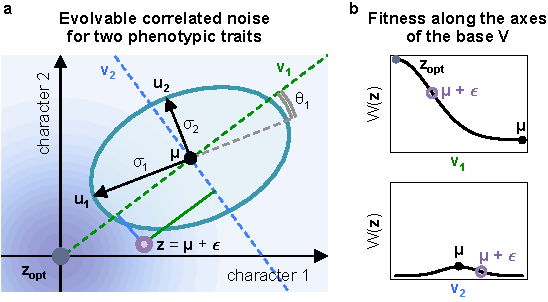
\includegraphics[scale=1.5]{part1_appendixS3_fig4.pdf}
\end{adjustwidth}
\caption[Anisotropic and correlated phenotypic noise for two traits.]{\textbf{Anisotropic and correlated phenotypic noise for two traits.}
\textbf{a,} The phenotypic distribution of an organism $(\boldsymbol{\mu}, \boldsymbol{\sigma}, \boldsymbol{\theta})$ is defined by a multivariate normal distribution with mean $\boldsymbol{\mu}$ (black dot), noise amplitudes $\sigma_1$ and $\sigma_2$ (black arrows) along axes $\boldsymbol{u_1}$ and $\boldsymbol{u_2}$, and a parameter of correlation $\theta_1$ (grey angle), defining a rotation of the basis $\boldsymbol{U} = (\boldsymbol{u_1}, \boldsymbol{u_2})$. A phenotype $\boldsymbol{z}$ (purple dot) is generated from the multivariate normal distribution by drawing a random vector $\boldsymbol{\epsilon} \sim \mathcal{N}_n(\boldsymbol{0},\boldsymbol{\Sigma})$ (with $\boldsymbol{\Sigma}$ the covariance matrix built from $\boldsymbol{\sigma}$ and $\boldsymbol{\theta}$), such that $\boldsymbol{z} = \boldsymbol{\mu} + \boldsymbol{\epsilon}$. The contribution of $\boldsymbol{\epsilon}$ on each axis $\boldsymbol{v_1}$ (in green) and $\boldsymbol{v_2}$ (in blue) of the basis $\boldsymbol{V}$, where $\boldsymbol{v_1}$ is aligned with the fitness optimum $\boldsymbol{z_{opt}}$, is represented by the vector $\boldsymbol{s} = (s_1, s_2)^T$. The fitness landscape is represented by a gradient of blue centered on the fitness optimum $\boldsymbol{z_{opt}}$ (blue dot).
\textbf{b,} Fitness along axes of the basis $\boldsymbol{V} = (\boldsymbol{v_1}, \boldsymbol{v_2})$. Along axis $\boldsymbol{v_1}$, aligned with the fitness optimum $\boldsymbol{z_{opt}}$, the organism experiences a convex fitness (if $\lVert \boldsymbol{\mu} \rVert > 1$). Along axis $\boldsymbol{v_2}$, orthogonal to $\boldsymbol{v_1}$, the organism a concave fitness, sitting on a local fitness optimum.
}
\label{part1:appendixS3:fig4}
\end{figure}

%%%%%%%%%%%%%%%%%
%%%%%%%%%%%%%%%%%

\section*{Concluding remarks}

Our demonstrations mainly rely on the study of the local convexity of the fitness function. As such, any function admitting the same properties as $W(\boldsymbol{z})=\exp\left[-\boldsymbol{z}^2/2\right]$ (\textit{i.e.}, a positive function being concave at the optimum and admitting one convex inflection point) will give the same general results. Moreover, in our study, phenotypic noise and mutation distributions are Gaussian-shaped. As demonstrated above, this choice allowed us to obtain precise analytical results.

